\subsection{TensorFlow graphs}

While the other discussed representations are familiar to most compiler developments,
one of key use cases for \MLIR is to support the development of machine
learning frameworks. Their internal representations is often based on a data
flow graph~\cite{veen} with a dynamic execution semantics.

TensorFlow~\cite{tensorflow2015-whitepaper} is an example of such framework.
Its representation is a high-level dataflow computation where the
nodes are computations which can be placed on various devices, including
specific hardware accelerators.

\MLIR is used in TensorFlow to model this internal representation and perform
transformations for the use cases presented in \figref{ml-compile}: from
simple algebraic optimizations to retargeting graphs
for parallel execution on data center clusters of hardware accelerators, from
lowering to a representation suitable for mobile deployment to
generating efficient native code using tools like XLA~\cite{xla}. The representation of
a TensorFlow graph in \MLIR is illustrated on~\figref{tf}.

\begin{figure}[t]
  \centering
  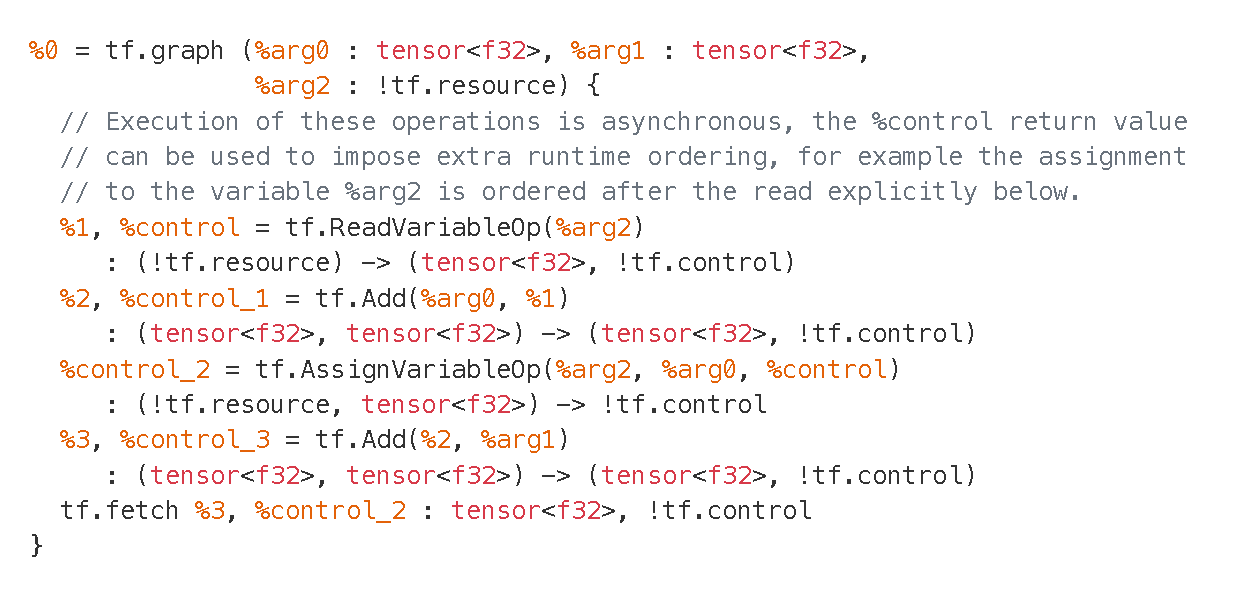
\includegraphics[width=.8\textwidth]{img/tf_mlir.pdf}
%\begin{tabular}{c}
%\begin{lstlisting}[language=mlir]
%%0 = tf.graph (%arg0 : tensor<f32>, %arg1 : tensor<f32>,
%               %arg2 : !tf.resource) {
% // Execution of these operations is asynchronous, the %control
% // return value can be used to impose extra runtime ordering,
% // for example the assignment to the variable %arg2 is ordered
% // after the read explicitly below.
% %1, %control = tf.ReadVariableOp(%arg2)
%     : (!tf.resource) -> (tensor<f32>, !tf.control)
% %2, %control_1 = tf.Add(%arg0, %1)
%     : (tensor<f32>, tensor<f32>) -> (tensor<f32>, !tf.control)
% %control_2 = tf.AssignVariableOp(%arg2, %2, %control)
%     : (!tf.resource, tensor<f32>) -> !tf.control
% %3, %control_3 = tf.Add(%2, %arg1)
%     : (tensor<f32>, tensor<f32>) -> (tensor<f32>, !tf.control)
% tf.fetch %3, %control_2 : tensor<f32>, !tf.control
%}
%
%\end{lstlisting}
%\end{tabular}
\caption{SSA representation of a TensorFlow dataflow graph in \MLIR.}\label{fig:tf}
\end{figure}

